\subsection{Ampersand as method} \label{Ampersand as method}
\def\cat{2}
The way of working with Ampersand requires preparation in the design and structuring of the work.
Experience plays a major role in this.
In the section on usefulnes (see~\ref{useful}) it was pointed out to maintain overview.
Keeping an overview helps when there are agreements about the naming of the Concepts, Relations and Rules.

\begin{table}[H]
    \caption{Category \acrshort{cat\cat}}
    \begin{tabularx}{\linewidth}{|X|X|}
        \hline
        Category        & CAT1-\cat \\\hline
        Category Title  & \acrshort{cat\cat} \\\hline
        Definition      & \acrlong{cat\cat} \\\hline
        Anchor examples & 
        \begin{itemize}
        \setlength{\itemindent}{-2em}
            \item \nameref{obs:rq1-25:12-9}
            \item \nameref{obs:rq1-80:20-11}
        \end{itemize}
        \\\hline
        Coding rules    & Approach and working with Ampersand \\\hline
    \end{tabularx}
    \label{tab:Ampersand as method}
\end{table}
\sbbs{1}{Naming}
\POstart{%1
    \POS{obs:rq1-30:12-9}     %\oref{obs:rq1-30:12-9}
    \POS{obs:rq1-33:14-9}     %\oref{obs:rq1-33:14-9}    x
    \POS{obs:rq1-38:3-10}     %\oref{obs:rq1-38:3-10}    x
    \POS{obs:rq1-46:24-10}     %\oref{obs:rq1-46:24-10}    x
    \POS{obs:rq1-80:20-11}     %\oref{obs:rq1-80:20-11}    x
    \POS{obs:rq2-4:30-9}     %\oref{obs:rq2-4:30-9}    o
    }

Having consistent naming conventions (\oref{obs:rq1-30:12-9}, \oref{obs:rq2-4:30-9}) in the scripts and thus in the conceptual design is important for readability (\oref{obs:rq1-80:20-11}).
Working with Includes and Patterns to get small delineated bits of functionality is important for overview (\oref{obs:rq1-33:14-9}, \oref{obs:rq1-38:3-10} ).
The agreements are also necessary to find concepts and relationships in the scripting.
Agreements are needed to be able to find Concepts and Relations in the script (\oref{obs:rq1-46:24-10}).
\sbbs{2}{Multiplicity}
\POstart{%2
    \POS{obs:rq1-3}     %\oref{obs:rq1-3}    x
    \POS{obs:rq2-2}     %\oref{obs:rq2-2}    x
    \POS{obs:rq1-21:7-11}     %\oref{obs:rq1-21:7-11}    x
    \POS{obs:rq1-58:8-11}     %\oref{obs:rq1-58:8-11}    x
    \POS{obs:rq2-11:19-10}     %\oref{obs:rq2-11:19-10}    x
    \POS{obs:rq2-12:19-10}     %\oref{obs:rq2-12:19-10}    x
    \POS{obs:rq2-13:19-10}     %\oref{obs:rq2-13:19-10}    x
    \POS{obs:rq2-5:2-10}     %\oref{obs:rq2-5:2-10}    x
}

In order to maintain an overview of the relations, an Excel sheet(see~\ref{fig:excel relation overview}) was drawn up in which the relations could be compiled (\oref{obs:rq2-5:2-10}, \oref{obs:rq1-3}, \oref{obs:rq2-11:19-10}).
This was to have support in the allocation of the multiplicities and was it possible to copy the relation definition to a script.
Noticed that only the UNI, TOT, INJ and SUR are used, where the UNI is mainly used and the TOT is often solved via a Rule.
The invariant violation prevents the prototype from storing data when multiple invariant violations occur simultaneously and that is when multiple TOT or SUR constraints are used (\oref{obs:rq1-21:7-11}, \oref{obs:rq2-12:19-10}, \oref{obs:rq2-13:19-10}, \oref{obs:rq1-58:8-11}).
\begin{figure}[H]
    \centering
    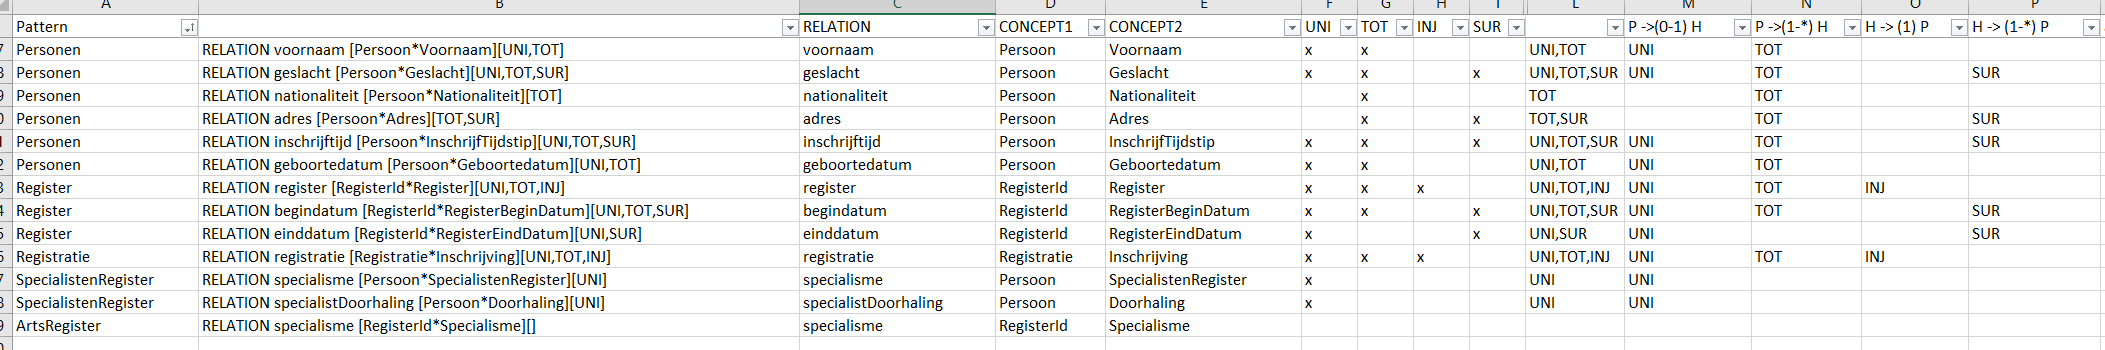
\includegraphics[width=1\textwidth]{excel relatie overzicht.PNG}
    \caption{excel relation overview}
    \label{fig:excel relation overview}
\end{figure}
%\newline\newline
\sbbs{3}{Rules}
\POstart{%3
    \POS{obs:rq1-4}     %\oref{obs:rq1-4}    x
    \POS{obs:rq1-61:9-11}     %\oref{obs:rq1-61:9-11}    x
    \POS{obs:rq1-63:10-11}     %\oref{obs:rq1-63:10-11}    x
    \POS{obs:rq1-67:11-11}     %\oref{obs:rq1-67:11-11}    x
    \POS{obs:rq2-19:16-11}     %\oref{obs:rq2-19:16-11}    x
    \POS{obs:rq2-6:2-10}     %\oref{obs:rq2-6:2-10}    x
}

The method Ampersand uses involves applying rules to relationships.
In concept the rules are easy to define, but in the Ampersand script a bit more difficult to construct (\oref{obs:rq1-4}, \oref{obs:rq2-6:2-10}).
It requires knowledge of Relation algebra to work with this correctly and it requires knowledge of Ampersand because it requires a certain way of notation (\oref{obs:rq1-63:10-11}).
Sometimes it seems logical to implement a rule, but there are implicit restrictions that make it unnecessary (\oref{obs:rq1-61:9-11}, \oref{obs:rq1-67:11-11}).
In the appendix \ref{appendixAdl} are examples of how to use Rules (\oref{obs:rq2-19:16-11}).
\sbbs{4}{Concept reuse}
\POstart{%4
    \POS{obs:rq1-79:20-11}     %\oref{obs:rq1-79:20-11}    x
    \POS{obs:rq1-91:14-12}     %\oref{obs:rq1-91:14-12}    x
}

The method allows multiple uses of the same Concepts and Relations (\oref{obs:rq1-91:14-12}, \oref{obs:rq1-79:20-11})
This is only visible when the documentation is generated.
By allowing the Concepts and Relationships multiple times, it is possible to add different definitions to them.
\sbbs{5}{Team}
\POstart{%5
    \PIS{int:I-1.4}     %\iref{int:I-1.4}    x
    \PIS{int:I-3.7}     %\iref{int:I-3.7}    x
    \PIS{int:I-4.13}     %\iref{int:I-4.13}    x
    \POS{obs:rq1-42:19-10}     %\oref{obs:rq1-42:19-10}    x
    \POS{obs:rq1-51:2-11}     %\oref{obs:rq1-51:2-11}    x
    \POS{obs:rq1-84:30-11}     %\oref{obs:rq1-84:30-11}    x
}

In addition to the technical approach, there is also a working method in which the user is closely involved.
In this case, it is important that a lawyer is involved at the start of the work to get a picture of the law (\iref{int:I-3.7}, \iref{int:I-1.4}).
Because Ampersand's approach to the definition is not very technical, a lawyer can easily understand this (\oref{obs:rq1-84:30-11}).
The \acrshort{ca} is also understandable for the lawyer.
It is therefore important to go through this theme (pattern) by theme (\oref{obs:rq1-51:2-11})
An analyst, as mentioned earlier, can perform this together with a lawyer (\iref{int:I-4.13}).
When processing it should not be forgotten that this information that is extracted from the \acrshort{big} is also directly processed in the script (\oref{obs:rq1-42:19-10})
\sbbs{6}{Prototype use}
\POstart{%6
    \PIS{int:I-2.11}     %\iref{int:I-2.11}    x
    \PIS{int:I-3.1}     %\iref{int:I-3.1}    x
    \PIS{int:I-3.2}     %\iref{int:I-3.2}    x
    \PIS{int:I-4.2}     %\iref{int:I-4.2}    x
    \POS{obs:rq1-57-1:7-11}     %\oref{obs:rq1-57-1:7-11}    x
    \PIS{int:I-1.8}     %\iref{int:I-1.8}    x    
}

We validate the data using the prototype and the \acrlong{ca} (\iref{int:I-1.8}).
During the research there was limited substantive validation, because the research focuses on the process and to a lesser extent on a validated design.
The conceptual analysis is labeled as understandable, recognizable and useful (\iref{int:I-3.1}, \iref{int:I-3.2}).
The prototype can be used to test the registry for the application of the law (\iref{int:I-2.11}).
Test cases can also be developed early in the development process on the basis of \acrshort{ca}.
The prototype was looked at through ICT glasses (\oref{obs:rq1-57-1:7-11}) and it turned out that it does not meet the \acrshort{cibg} requirements for a website.
The tutorials indicate that this is possible by means of a CSS adjustment, but how exactly this should be done is not entirely clear and is also outside the scope of this research (\iref{int:I-4.2}).
\sbbs{7}{Organisation Ampersand use}
\POstart{%7
    \PIS{int:I-1.1}     %\iref{int:I-1.1}    x
    \PIS{int:I-1.9}     %\iref{int:I-1.9}    x
    \PIS{int:I-4.10}     %\iref{int:I-4.10}    x
    \PIS{int:I-4.14}     %\iref{int:I-4.14}    x
}

Ampersand's acknowledgment as instigator of real-time signal violations is not reflected in the interviews.
It is expected that Ampersand can be used in the preliminary phase of the design (\iref{int:I-4.14}).
There was also the expectation that Ampersand would be able to independently process texts into scripts (\iref{int:I-1.1})
Within the organization people are used to working according to fixed processes, the reactive approach of Ampersand is therefore not always immediately understood (\iref{int:I-1.9}).
Ampersand's method focuses on text analysis and from there on models (\iref{int:I-4.10}) as opposed to methods that work from the models.
\sbbs{8}{Excluded}
\POstart{%8
    \PIS{int:I-4.5}     %\iref{int:I-4.5}    o
    \PIS{int:I-4.9}     %\iref{int:I-4.9}    o
    \POS{obs:rq1-55:2-11}     %\oref{obs:rq1-55:2-11}    o
    \POS{obs:rq1-7:10-11}     %\oref{obs:rq1-7:10-11}    o
    \POS{obs:rq1-90:14-12}     %\oref{obs:rq1-90:14-12}    o
    \POS{obs:rq2-10:19-10}     %\oref{obs:rq2-10:19-10}    o
    \POS{obs:rq2-14:19-10}     %\oref{obs:rq2-14:19-10}    o
    \POS{obs:rq2-8:7-10}     %\oref{obs:rq2-8:7-10}    o
}

The following observations have not been explicitly included.

